\documentclass[tikz,border=10pt,12pt,x11names]{standalone}
\usepackage{verbatim}
%%%>
\usetikzlibrary{calc,arrows}
\usepackage{tikz}
\usepackage[]{circuitikz} % TiKZ Library for US Logic Circuits.
\usetikzlibrary{circuits.logic.US} % TiKZ Library for US Logic Circuits.
\usepackage{amsmath}

\usepackage{tikz}
\usetikzlibrary{circuits.logic.US} % TiKZ Library for US Logic Circuits.
\begin{document}

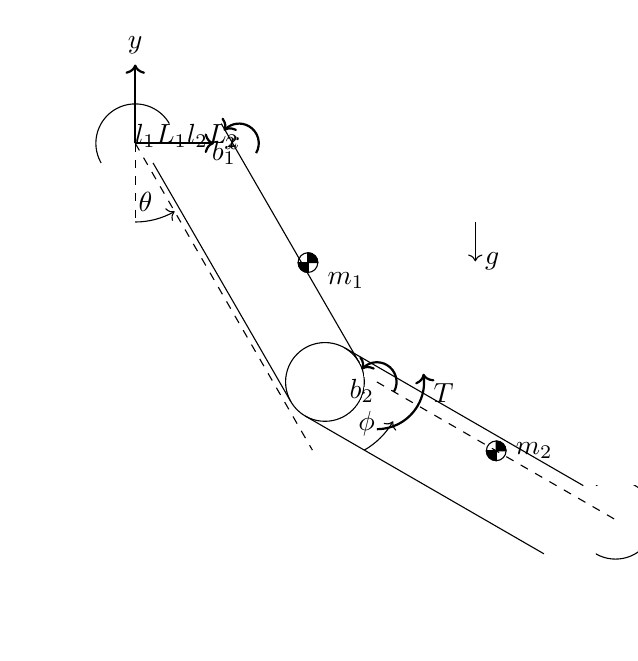
\begin{tikzpicture}[scale=0.5]

\begin{scope}
\clip [rotate=30] (-2,0) rectangle (2,2);
\draw (0,0) circle [radius=1cm];
\end{scope}

\coordinate (O) at (0,0) ;
% Second cirle middle point
\coordinate (A) at (3.5,-6.06217); 
\coordinate (B) at (3.5+6.06217,-6.06217-3.5); 
% Lenght of pendulums are 7cm

% Axis for underactuated Pendulum
\draw[->,thick] (0,0) -- (2,0) node[anchor=west] {$x$};
\draw[->,thick] (0,0) -- (0,2) node[anchor=south] {$y$};
\draw[dashed] (0,0) -- (0,-2);

%%%%%%%%%%%%%%%%%%%%%%%%%%%%%%%%%%%%%%%%%%%%%%%%%%%%%%%%%%%%%%%%%%%%%%%%%%%%%%
%% Theta %%
\begin{scope}
\draw[->] (0,-2) arc (270:300:2);
\draw (280:1.5) node {$\theta$};
\end{scope}
%%%%%%%%%%%%%%%%%%%%%%%%%%%%%%%%%%%%%%%%%%%%%%%%%%%%%%%%%%%%%%%%%%%%%%%%%%%%%%

%%%%%%%%%%%%%%%%%%%%%%%%%%%%%%%%%%%%%%%%%%%%%%%%%%%%%%%%%%%%%%%%%%%%%%%%%%%%%%
%% Middle line for underactuated pendulum %%
\draw[dashed] (0,0) -- (4.5,-7.79422);
%%%%%%%%%%%%%%%%%%%%%%%%%%%%%%%%%%%%%%%%%%%%%%%%%%%%%%%%%%%%%%%%%%%%%%%%%%%%%%


%%%%%%%%%%%%%%%%%%%%%%%%%%%%%%%%%%%%%%%%%%%%%%%%%%%%%%%%%%%%%%%%%%%%%%%%%%%%%%
%% Dimensions of underactuated Pendulum %%
\dimline[line style = {line width=0.7},extension start length=-0.25, extension end length=-0.4]{(-1.732,-1)}{(-1.732+1.75,-1-3.031)}{$l_{1}$}

\dimline[line style = {line width=0.7},extension start length=-0.25, extension end length=-0.25]{(-2.598,-1.5)}{(-2.598+3.5,-1.5-6.06217)}{$L_{1}$}

%%%%%%%%%%%%%%%%%%%%%%%%%%%%%%%%%%%%%%%%%%%%%%%%%%%%%%%%%%%%%%%%%%%%%%%%%%%%%%

%Long lines for underactuated pendulum
\draw (0.8660,0.5) -- (0.866+3.5,0.5-6.06217);
\draw (-0.8660,-0.5) -- (-0.866+3.5,-0.5-6.06217);	



%%%%%%%%%%%%%%%%%%%%%%%%%%%%%%%%%%%%%%%%%%%%%%%%%%%%%%%%%%%%%%%%%%%%%%%%%%%%%%
%% Middle circle for both pendulums %%
\begin{scope}
%\clip [rotate=00] (0.866+3.5,0.5-6.06217+2) rectangle (-0.866+3.5-2,-0.5-6.06217);
\clip (A) circle [radius=1.02];
\draw (A) circle [radius=1cm];
\end{scope}

%\draw [rotate=00] (0.866+3.5,0.5-6.06217+2) rectangle (-0.866+3.5-2,-0.5-6.06217);

%%%%%%%%%%%%%%%%%%%%%%%%%%%%%%%%%%%%%%%%%%%%%%%%%%%%%%%%%%%%%%%%%%%%%%%%%%%%%%
% Axis for lower Pendulum
%\draw[->,thick] (3.5,-6.06217) -- (6.5,-6.06217) node[anchor=west] {$x_{2}$};
%\draw[->,thick] (3.5,-6.06217) -- (3.5,-3.06217) node[anchor=south] {$y_{2}$};
%\draw[dashed] (3.5,-6.06217) -- (3.5,-8.56217);

% Long lines for actuated pendulum
\draw (3.5+0.5,-6.06217+0.86602) -- (3.5+0.5+6.06217,-6.06217+0.86602-3.5);
\draw (3.5-0.5,-6.06217-0.86602) -- (3.5-0.5+6.06217,-6.06217-0.86602-3.5);

%%%%%%%%%%%%%%%%%%%%%%%%%%%%%%%%%%%%%%%%%%%%%%%%%%%%%%%%%%%%%%%%%%%%%%%%%%%%%%
%%  Phi %%
\begin{scope}
\draw[->] (4.5,-7.79422) arc (300:330:2);


\draw (3.5,-6.06217)+ (315:1.5) node {$\phi$};
\end{scope}
%%%%%%%%%%%%%%%%%%%%%%%%%%%%%%%%%%%%%%%%%%%%%%%%%%%%%%%%%%%%%%%%%%%%%%%%%%%%%%

%%%%%%%%%%%%%%%%%%%%%%%%%%%%%%%%%%%%%%%%%%%%%%%%%%%%%%%%%%%%%%%%%%%%%%%%%%%%%%
%% Dimensions of actuated Pendulum %%
\dimline[line style = {line width=0.7},extension start length=-0.25, extension end length=-0.4]{(2.5,-7.79421)}{(5.53108,-9.54422)}{$l_{2}$}

\dimline[line style = {line width=0.7},extension start length=-0.25, extension end length=-0.25]{(2,-8.66028)}{(8.06217,-12.1602)}{$L_{2}$}

%%%%%%%%%%%%%%%%%%%%%%%%%%%%%%%%%%%%%%%%%%%%%%%%%%%%%%%%%%%%%%%%%%%%%%%%%%%%%%


%%%%%%%%%%%%%%%%%%%%%%%%%%%%%%%%%%%%%%%%%%%%%%%%%%%%%%%%%%%%%%%%%%%%%%%%%%%%%%
%% Circle at the bottom %%
\begin{scope}
\clip [rotate=00] (3.5+0.5+6.06217+2,-6.06217+0.86602-3.5) rectangle ((3.5-0.5+6.06217,-6.06217-0.86602-3.5-2);
\draw (B) circle [radius=1cm];
\end{scope}
%%%%%%%%%%%%%%%%%%%%%%%%%%%%%%%%%%%%%%%%%%%%%%%%%%%%%%%%%%%%%%%%%%%%%%%%%%%%%%


%%%%%%%%%%%%%%%%%%%%%%%%%%%%%%%%%%%%%%%%%%%%%%%%%%%%%%%%%%%%%%%%%%%%%%%%%%%%%%
%% Middle line for actuated pendulum %%
\draw[dashed] (3.5,-6.06217)--(3.5+6.06217,-6.06217-3.5);
%%%%%%%%%%%%%%%%%%%%%%%%%%%%%%%%%%%%%%%%%%%%%%%%%%%%%%%%%%%%%%%%%%%%%%%%%%%%%%

%%%%%%%%%%%%%%%%%%%%%%%%%%%%%%%%%%%%%%%%%%%%%%%%%%%%%%%%%%%%%%%%%%%%%%%%%%%%%%
%% Centroid symbol for underactuade pendulum %%
\draw (1.75,-3.0310) circle [radius=0.25cm];
\draw (1.75-0.25,-3.0310) -- (1.75+0.25,-3.0310)  node[below right]{$m_{1}$};`
\draw (1.75,-3.0310+0.25) -- (1.75,-3.0310-0.25);
\filldraw[fill=black,draw=black] (1.75,-3.0310) -- (1.75+0.25,-3.0310)
arc[start angle = 0, end angle = 90, radius = 0.25] -- cycle;

\filldraw[fill=black,draw=black] (1.75,-3.0310) -- (1.75-0.25,-3.0310)
arc[start angle = 180, end angle = 270, radius = 0.25] -- cycle ;
%%%%%%%%%%%%%%%%%%%%%%%%%%%%%%%%%%%%%%%%%%%%%%%%%%%%%%%%%%%%%%%%%%%%%%%%%%%%%%

%%%%%%%%%%%%%%%%%%%%%%%%%%%%%%%%%%%%%%%%%%%%%%%%%%%%%%%%%%%%%%%%%%%%%%%%%%%%%%
%% Centroid symbol for actuaded pendulum %%
\draw (6.53108,-7.81217) circle [radius=0.25cm];
\draw (6.53108-0.25,-7.81217) -- (6.53108+0.25,-7.81217)  node[right]{$m_{2}$};
\draw (6.53108,-7.81217+0.25) -- (6.53108,-7.81217-0.25);
\filldraw[fill=black,draw=black] (6.53108,-7.81217) -- (6.53108+0.25,-7.81217)
arc[start angle = 0, end angle = 90, radius = 0.25] -- cycle;

\filldraw[fill=black,draw=black] (6.53108,-7.81217) -- (6.53108-0.25,-7.81217)
arc[start angle = 180, end angle = 270, radius = 0.25] -- cycle ;
%%%%%%%%%%%%%%%%%%%%%%%%%%%%%%%%%%%%%%%%%%%%%%%%%%%%%%%%%%%%%%%%%%%%%%%%%%%%%%

% Torque Input
%\draw[->,thick] (3.5,-7.5) to [bend right] (5.25,-4.76314) node[right]{$T$}; 
\draw[->,thick] (A) +(0,-1.2) arc (270:370:1.2) node[below right] {$T$};


% Damping in bearings
\draw[->,thick] (0.433,-0.25) arc (330:500:0.5) node[below] {$b_{1}$};

% Damping between motor rotor and stator 
\draw[->,thick] (A)+(0.433,-0.25) arc (330:500:0.5) node[below] {$b_{2}$};

% Direction of gravity
\draw[->] (6,-2)--(6,-3) node[right]{$g$};

% Labels for pendulums

\end{tikzpicture}
\end{document}